%% BioMed_Central_Tex_Template_v1.06
%%                                      %
%  bmc_article.tex            ver: 1.06 %
%                                       %

%%IMPORTANT: do not delete the first line of this template
%%It must be present to enable the BMC Submission system to
%%recognise this template!!

%%%%%%%%%%%%%%%%%%%%%%%%%%%%%%%%%%%%%%%%%
%%                                     %%
%%  LaTeX template for BioMed Central  %%
%%     journal article submissions     %%
%%                                     %%
%%          <8 June 2012>              %%
%%                                     %%
%%                                     %%
%%%%%%%%%%%%%%%%%%%%%%%%%%%%%%%%%%%%%%%%%


%%%%%%%%%%%%%%%%%%%%%%%%%%%%%%%%%%%%%%%%%%%%%%%%%%%%%%%%%%%%%%%%%%%%%
%%                                                                 %%
%% For instructions on how to fill out this Tex template           %%
%% document please refer to Readme.html and the instructions for   %%
%% authors page on the biomed central website                      %%
%% http://www.biomedcentral.com/info/authors/                      %%
%%                                                                 %%
%% Please do not use \input{...} to include other tex files.       %%
%% Submit your LaTeX manuscript as one .tex document.              %%
%%                                                                 %%
%% All additional figures and files should be attached             %%
%% separately and not embedded in the \TeX\ document itself.       %%
%%                                                                 %%
%% BioMed Central currently use the MikTex distribution of         %%
%% TeX for Windows) of TeX and LaTeX.  This is available from      %%
%% http://www.miktex.org                                           %%
%%                                                                 %%
%%%%%%%%%%%%%%%%%%%%%%%%%%%%%%%%%%%%%%%%%%%%%%%%%%%%%%%%%%%%%%%%%%%%%

%%% additional documentclass options:
%  [doublespacing]
%  [linenumbers]   - put the line numbers on margins

%%% loading packages, author definitions

%\documentclass[twocolumn]{bmcart}% uncomment this for twocolumn layout and comment line below
\documentclass{bmcart}

%%% Load packages
%\usepackage{amsthm,amsmath}
%\RequirePackage{natbib}
%\RequirePackage[authoryear]{natbib}% uncomment this for author-year bibliography
%\RequirePackage{hyperref}
\usepackage[utf8]{inputenc} %unicode support
%\usepackage[applemac]{inputenc} %applemac support if unicode package fails
%\usepackage[latin1]{inputenc} %UNIX support if unicode package fails
\usepackage{mathtools}
\usepackage[pdf]{graphviz}

% code listings
\usepackage{listings}
%%%%%%%%%%%%%%%%%%%%%%%%%%%%%%%%%%%%%%%%%%%%%%%%%
%%                                             %%
%%  If you wish to display your graphics for   %%
%%  your own use using includegraphic or       %%
%%  includegraphics, then comment out the      %%
%%  following two lines of code.               %%
%%  NB: These line *must* be included when     %%
%%  submitting to BMC.                         %%
%%  All figure files must be submitted as      %%
%%  separate graphics through the BMC          %%
%%  submission process, not included in the    %%
%%  submitted article.                         %%
%%                                             %%
%%%%%%%%%%%%%%%%%%%%%%%%%%%%%%%%%%%%%%%%%%%%%%%%%


\def\includegraphic{}
\def\includegraphics{}



%%% Put your definitions there:
\startlocaldefs
\endlocaldefs


%%% Begin ...
\begin{document}

%%% Start of article front matter
\begin{frontmatter}

\begin{fmbox}
\dochead{Research}

%%%%%%%%%%%%%%%%%%%%%%%%%%%%%%%%%%%%%%%%%%%%%%
%%                                          %%
%% Enter the title of your article here     %%
%%                                          %%
%%%%%%%%%%%%%%%%%%%%%%%%%%%%%%%%%%%%%%%%%%%%%%

\title{A hybrid P. Falciparum transmission model}

%%%%%%%%%%%%%%%%%%%%%%%%%%%%%%%%%%%%%%%%%%%%%%
%%                                          %%
%% Enter the authors here                   %%
%%                                          %%
%% Specify information, if available,       %%
%% in the form:                             %%
%%   <key>={<id1>,<id2>}                    %%
%%   <key>=                                 %%
%% Comment or delete the keys which are     %%
%% not used. Repeat \author command as much %%
%% as required.                             %%
%%                                          %%
%%%%%%%%%%%%%%%%%%%%%%%%%%%%%%%%%%%%%%%%%%%%%%

\author[
   addressref={aff1},                   % id's of addresses, e.g. {aff1,aff2}
   corref={aff1},                       % id of corresponding address, if any
   noteref={n1},                        % id's of article notes, if any
   email={giovanni.charles10@imperial.ac.uk}   % email address
]{\inits{GC}\fnm{Giovanni} \snm{Charles}}

% TODO: other authors (Ellie, Azra)
%\author[
%   addressref={aff1,aff2},
%   email={john.RS.Smith@cambridge.co.uk}
%]{\inits{PW}\fnm{Peter} \snm{Winskill}}

%%%%%%%%%%%%%%%%%%%%%%%%%%%%%%%%%%%%%%%%%%%%%%
%%                                          %%
%% Enter the authors' addresses here        %%
%%                                          %%
%% Repeat \address commands as much as      %%
%% required.                                %%
%%                                          %%
%%%%%%%%%%%%%%%%%%%%%%%%%%%%%%%%%%%%%%%%%%%%%%

\address[id=aff1]{%                           % unique id
  \orgname{Department of Infectious Disease, Imperial College London}, % university, etc
  \street{Praed Street},                      %
  %\postcode{}                                % post or zip code
  \city{London},                              % city
  \cny{UK}                                    % country
}
%\address[id=aff2]{%
%  \orgname{Marine Ecology Department, Institute of Marine Sciences Kiel},
%  \street{D\"{u}sternbrooker Weg 20},
%  \postcode{24105}
%  \city{Kiel},
%  \cny{Germany}
%}

%%%%%%%%%%%%%%%%%%%%%%%%%%%%%%%%%%%%%%%%%%%%%%
%%                                          %%
%% Enter short notes here                   %%
%%                                          %%
%% Short notes will be after addresses      %%
%% on first page.                           %%
%%                                          %%
%%%%%%%%%%%%%%%%%%%%%%%%%%%%%%%%%%%%%%%%%%%%%%

\begin{artnotes}
%\note{Sample of title note}     % note to the article
\note[id=n1]{Equal contributor} % note, connected to author
\end{artnotes}

\end{fmbox}% comment this for two column layout

%%%%%%%%%%%%%%%%%%%%%%%%%%%%%%%%%%%%%%%%%%%%%%
%%                                          %%
%% The Abstract begins here                 %%
%%                                          %%
%% Please refer to the Instructions for     %%
%% authors on http://www.biomedcentral.com  %%
%% and include the section headings         %%
%% accordingly for your article type.       %%
%%                                          %%
%%%%%%%%%%%%%%%%%%%%%%%%%%%%%%%%%%%%%%%%%%%%%%

\begin{abstractbox}

\begin{abstract} % abstract
\parttitle{Background}
With the quick development of Malaria epidemiology, we need to take into account a growing list of factors to keep our studies applicable, including vector behaviours, human immunity, seasonality, and combined interventions. Studying these complex dynamics can be made easier with an up-to-date, flexible, integrated model of Malaria transmission.

\parttitle{Methods}
We constructed model of P. Falciparum transmission which is highly configurable through the R-based interface. The implementation is divided into an individual-based model of human transmission and a compartmental model for the vector life-cycle and transmission.

\parttitle{Results}
The code is made available as a public package for use in the community. It builds on recent integrated models by including updated bed net and transmission blocking vaccine models, and is in active development to integrate more dynamics.

We recreated the outputs from previous studies to verify the consistency between transmission models.

\parttitle{Conclusions}
This model provides an easy method for studying a variety of scenarios or calibrating parameters to data. The structure of the model also simplifies the introduction of new research into an existing model.

\end{abstract}

%%%%%%%%%%%%%%%%%%%%%%%%%%%%%%%%%%%%%%%%%%%%%%
%%                                          %%
%% The keywords begin here                  %%
%%                                          %%
%% Put each keyword in separate \kwd{}.     %%
%%                                          %%
%%%%%%%%%%%%%%%%%%%%%%%%%%%%%%%%%%%%%%%%%%%%%%

\begin{keyword}
\kwd{Individual-based model}
\kwd{Agent-based model}
\kwd{Compartmental}
\kwd{P. Falciparum}
\end{keyword}

% MSC classifications codes, if any
%\begin{keyword}[class=AMS]
%\kwd[Primary ]{}
%\kwd{}
%\kwd[; secondary ]{}
%\end{keyword}

\end{abstractbox}
%
%\end{fmbox}% uncomment this for twcolumn layout

\end{frontmatter}

%%%%%%%%%%%%%%%%%%%%%%%%%%%%%%%%%%%%%%%%%%%%%%
%%                                          %%
%% The Main Body begins here                %%
%%                                          %%
%% Please refer to the instructions for     %%
%% authors on:                              %%
%% http://www.biomedcentral.com/info/authors%%
%% and include the section headings         %%
%% accordingly for your article type.       %%
%%                                          %%
%% See the Results and Discussion section   %%
%% for details on how to create sub-sections%%
%%                                          %%
%% use \cite{...} to cite references        %%
%%  \cite{koon} and                         %%
%%  \cite{oreg,khar,zvai,xjon,schn,pond}    %%
%%  \nocite{smith,marg,hunn,advi,koha,mouse}%%
%%                                          %%
%%%%%%%%%%%%%%%%%%%%%%%%%%%%%%%%%%%%%%%%%%%%%%

%%%%%%%%%%%%%%%%%%%%%%%%% start of article main body
% <put your article body there>

%%%%%%%%%%%%%%%%
%% Background %%
%%
\section*{Background}

The detailed mathematical model of P. Falicparum transmission specified in \cite{griffin_reducing_2010}, became the foundation for several updates, extensions and studies in the following years. It took into account immunity dynamics, seasonality, a vector feeding and reproduction cycle, anti-malarial treatments, bed nets, indoor residual spraying and mass drug administration.

Since then, \cite{okell_contrasting_2014} published models for a variety of Artemisinin-combination therapies. These included a continuous model for prophylaxis.

Later, \cite{white_immunogenicity_2015} introduced an antibody model of RTS,S. Accounting for antibody titres better characterised the immugenicity of an individual.

In \cite{griffin_is_2016}, Jamie Griffin outlines a method for finding the equilibrium of his model. This greatly reduces the warm-up time needed for simulations. 

A systematic review of indoor residual spraying by \cite{sherrard-smith_systematic_2018}, lead to new models for vector control. The updated models account for the impact of vector controls on vector mortality, feeding attempts and deterrence in the face of insecticide resistance.

Recent efforts have explored a hypothetical transmission-blocking vaccine \cite{challenger_predicting_2021}. Predictive studies like these could steer pharmaceutical development towards effective new tools for reducing the burden of Malaria.

We present the latest model which captures the recent progress Malaria transmission dynamics. It is a flexible, modular, highly configurable model for simulating detailed intervention strategies.

\section*{Methods}

The model is made up of four main components, shown in figure[]. Each requires limited interactions with the others, allowing for flexibility and specialisation in the implementations. The compartmental vector models are implemented with an Ordinary Differential Equation (ODE) solver using the Dormand-Prince method, while the human model is implemented as an individual-based model. There are two interchangeable implementations of the adult mosquito model. An individual-based implementation allows for fine grained modelling, whereas the compartmental implementation trades detail for execution speed.

\begin{figure}[h]
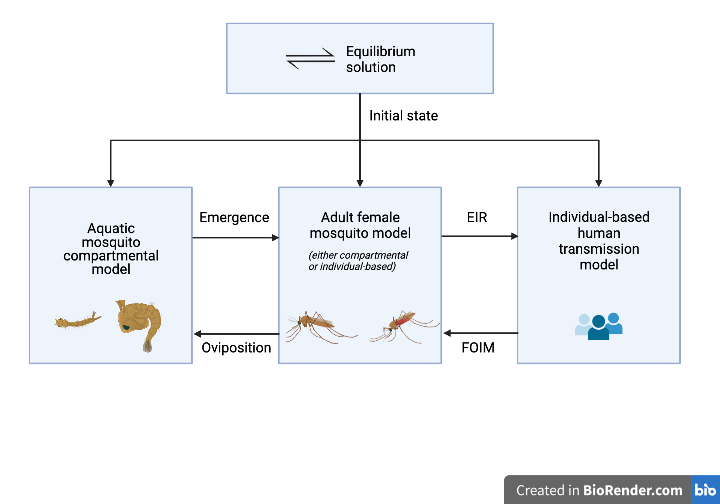
\includegraphics[width=8cm]{Malariasimulation.png}
\end{figure}

\subsection*{Vector models}

The aquatic mosquito model is an ordinary differential equation model determining adult mosquito emergence, shown in figure[]. The first compartment $(E)$ represents the early stage larvae. Their births are governed by the total number of mosquitoes in the adult model. Both the early and late $(L)$ stage compartments have density dependent death rates, as shown in equation[]. The carrying capacity of a site is modelled based on rainfall profiles.

The adult mosquito model is a system of delay differential equations determining the EIR of the model. Susceptible mosquitoes $(S_m)$ are infected at rate $\Lambda_m$ or the Force Of Infection towards Mosquitoes \(FOIM\). Before becoming infectious, they undergo an extrinsic incubation period of length $\tau$ in the $E_m$ compartment. After which they will remain infectious until death.

The individual counterpart for the adult mosquito model samples infection as a bernoulli trail. The success probability of each trail is determined by $\Lambda_m$.

\subsection*{Human transmission model}

The human model works on the individual level to estimate Malaria prevalence statistics. The model is outlined in figure[]. Susceptible humans are exposed to infectious bites at a rate $\Lambda$, the EIR. The first like of defence is pre-erythrocytic immunity (IB). The probability of infection given a bite is shown in []. We subsequently model an immunity to clinical infection (IC), which influences the probability of an asymptomatic infection. Clinical infections can be avoided with treatment with probability $f_t$ resulting in a transition to $Tr$, or $D$ if untreated. Individuals in the $A$ and $U$ state can be super-infected, prolonging their time spent in a diseased state. State transitions are sampled every time step as bernoulli trials with the following probabilities:

%TODO: table

\begin{figure}[h]
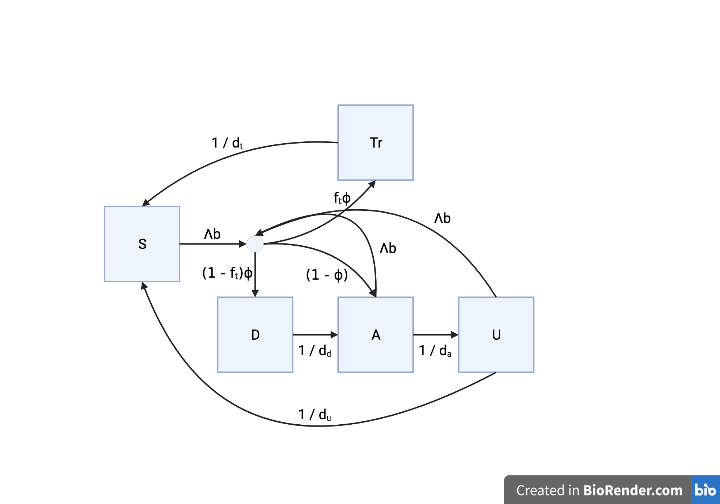
\includegraphics[width=8cm]{Human state transition.png}
\end{figure}

\subsection*{Equilibrium solution}

The equilibrium solution can be used on its own to calculate the steady state values of the aquatic, adult female mosquitoes and human Malaria transmission models for a given EIR. For the vector models, it is used to initialise the size of the $E,L,P,S_m,E_m,I_m$ compartments. For the human transmission model, humans are binned into age and heterogeneity group to match the compartments of the equilibrium solution. Their infection states $S,D,A,U,Tr$ are sampled based on the relative size of each compartment. They are also assigned mean immunity levels $IB,ICA,ICM,IVA,IVM,ID$ for their corresponding compartments.

These values are intended as starting points. The complete model has continuous values for heterogeneity and age, and models seasonal mosquito density, and so may converge on slightly different steady states.

\subsection*{Treatment}

Pharmacological treatment affects Malaria transmission in three ways:
\begin{itemize}
    \item Reduction in clinical infection. If clinical immunity fails an individual can be treated to move them to the treated state (Tr) instead of the D state. Treated individuals are included in the incidence statistics but contribute no infectiousness towards mosquitoes. The probability of a treatment attempt, or treatment coverage per drug over time, is $\text{cov}_d(t)$. The probability of successfully treating an individual is $\text{eff}_d$. When an individual is about to be clinically infected, a treatment attempt and treatment success are modelled as successive Bernoulli trials with probabilities $\text{cov}_d(t)$ and $\text{eff}_d$ respectively.
    \item Prophylaxis. Following treatment, individuals will have a reduced probability of erythrocytic infection. The reduction is determined by a Weibull survival curve with shape and scale parameters $\lambda_d$, $\kappa_d$
    \item Reduced infectiousness towards mosquitoes. The infectiousness of treated individuals will be reduced by a factor of $rel\_c_d$
\end{itemize}

Parameter values for for $\text{eff}_d$, $\lambda_d$, $\kappa_d$ and $rel\_c_d$ have been estimated for a variety of anti-malarial drugs, including Artemisinin-based combination therapies in \cite{okell_contrasting_2014} TODO cite more.

We can also model a mass drug administration on a sub-population. A sub-population can be specified by age range, coverage per time step and correlation parameters.

\subsection*{Vector controls}

The two vector controls included in the simulation are bed nets and indoor residual spraying. Both of these interventions affect the mortality and biting rates for each species of mosquito.

The mortality rate is increased when mosquitoes come into contact with insecticide, either on a net or on a sprayed surface. We can express a dynamic mortality rate $mu_v$ as a function of the feeding rate $f^v_R$ and the probabilities of surviving feeding $p^v_1$ and the gonotrophic cycle $p^v_2$.

\[
\mu^v = -f_R^v \log(p_1^vp_2^v)
\]

Without vector controls, we model the probability of surviving a feeding attempt as $p_{10}^v$, a function of the natural time spent in search of a blood meal, $\delta_{10}^v$ and the natural mortality rate for a vector, $\mu_0^v$:

\[
p_{10}^v = \exp(-\mu_0^v\delta^v_{10})
\]

As vector controls are introduced, $p_1^v$ will become less than $p_{10}^v$. This is because vectors will have a smaller probability of a successful feeding attempt, $W^v$, and have a larger probability of being repelled $Z^v$. We can express $p_1^v$ as:

\[
p_1^v = \frac{p_{10}^vW^v}{1 - Z^vp^v_{10}}
\]

$p_2^v$ will remain independent of vector controls as we can express it as a function of $\mu_0^v$ and the time for each species' gonotrophic cycle, $\delta_2^v$:

\[
p_2^v = \exp(-\mu_0^v\delta^v_2)
\]

Vector controls reduce the effective biting rate on each human $\lambda_i^v$ based on their level of protection. We can express $\lambda_i^v$ in terms of the human blood meal rate $\alpha^v$, the relative proportion of bites taken on each human $\pi_i$, the probability of a successful feeding attempt on the $i^{\text{th}}$ individual $w_i$ and the probability of feeding \emph{and} surviving on the $i^{\text{th}}$ individual $y_i$.

\[
\lambda_i^v = \frac{\alpha^v\pi_i y_i^v}{\sum\pi_i w_i^v}
\]

The human blood meal rate is a product of the overall blood meal rate $f_R^v$ and the proportion of blood meals taken on humans $Q^v$.

\[
\alpha^v = f_R^v Q^v
\]

In the face of vector controls, $f_R^v$ is reduced. This is because mosquitoes are repelled from and require a longer time to successfully find a blood meal, $\delta_1$. We can capture this extension in terms of the natural time take to find a blood meal $\delta_{10}$ and $Z^v$.

\[
f_R^v = \frac{1}{\delta^v_1 + \delta^v_2}
\]

Where,

\[
\delta^v_1 = \frac{\delta^v_10}{1 + Z^v}
\]

$Q^v$ is also reduced. Since fewer bites are successfully made on humans. We can capture that reduction in terms of the natural proportion of bites made on humans $Q^v_0$.

\[
Q^v = 1 - \frac{1 - Q^v_0}{W^v}
\]

Probabilities for $w_i$, $y_i$ and $z_i$, take in to account the level of protection that nets or spraying provide for each individual. When an individual has a net, the probability of a mosquito successfully feeding and being repelled on feeding attempt of host $i$ is $s_N$ and $r_N$ respectively. We define $s_S$ and $r_S$ for individuals who are protected by indoor residual spraying. The proportion of feeding attempts indoors and on hosts in bed are $\Phi_I$ and $\Phi_B$ respectively.

\begin{gather*}
    w_i = 1 - \Phi_I + \Phi_B(1 -  r_S)s_Ns_S + (\Phi_I - \Phi_B)(1 - r_S)s_S\\
    y_i = 1 - \Phi_I + \Phi_B(1 -  r_S)s_N + (\Phi_I - \Phi_B)(1 - r_S)\\
    z_i = \Phi_B(1 - r_S)r_N + \Phi_Ir_S
\end{gather*}

For bed nets, $r_N$ and $s_N$ are estimated from bioassay data \cite{sherrard-smith_systematic_2018}. The effectiveness of the net in repelling mosquitoes is modelled as an exponential decay with rate $\gamma_N$ and scaled between minimum and maximum values $r_{NM}$ and $r_{N0}$. $s_N$ is modelled using $r_N$ and an intermediate value $d_N$, which represents the effectiveness of the net in killing mosquitoes. $d_N$ also has an exponential decay with rate $\gamma_N$. If an individual does not have a net, we can set $\Phi_B = r_N = 0, s_N = 1$ to remove the effects of nets from the equations for $w_i, y_i, z_i$.

\begin{gather*}
    s_N = 1 - r_N - d_N \\
    r_N = (r_{N0} - r_{NM})\exp(-t\gamma_N) + r_{NM} \\
    d_N = d_{N0}\exp(-t\gamma_N)
\end{gather*}

For indoor spraying, $r_S$ and $s_S$ are modelled in terms of experimental hut trial fits for logistic functions for vector mortality $l_s$, blood feeding rate $k_s$ and deterrence $m_s$ \cite{sherrard-smith_systematic_2018}. To capture the reduction in insecticide effectiveness over time, we use the estimate for $m_s$ to augment $l_s$ and $k_s$. If IRS is disabled, we set $\Phi_I = r_S = 0, s_S = 1$ to remove the effects of spraying from the equations for $w_i, y_i, z_i$.

\begin{gather*}
    s_S = \frac{k^\prime_S}{k_0} \\
    r_S = \left(1 - \frac{k^\prime_S}{k_0}\right)\left(\frac{j^\prime_S}{j^\prime_S + l^\prime_S}\right) \\
\end{gather*}

Where,

\begin{gather*}
    l_s = \frac{1}{1 + \exp(-(l_{S\theta} + l_{S\gamma} t))}\\
    k_s = \frac{1}{1 + \exp(-(k_{S\theta} + k_{S\gamma} t))}\\
    m_s = \frac{1}{1 + \exp(-(m_{S\theta} + m_{S\gamma} t))}
    j_s = 1 - l_s - k_s
\end{gather*}

And when augmented by deterrence we have,

\begin{gather*}
    l_s^\prime = l_s (1 - m_s)\\
    k_s^\prime = k_s (1 - m_s)\\
    j_s^\prime = j_s (1 - m_s) + m_s
\end{gather*}

Finally, the population-wide probabilities for $W^v$ and $Z^v$ can be aggregated from the individual level probabilities as follows:

\begin{gather*}
W^v = 1 - Q^v_0 + Q^v_0 \sum\pi_iw_i\\
Z^v = Q^v_0 \sum\pi_iz_i
\end{gather*}

\subsection*{Vaccination}

The RTS,S vaccine reduces the probability of pre-erythrocytic infection. The efficacy of the vaccine is modelled as a function of the antibodies it induces.

\[
V(t) = V_{max}\left(1 - \frac{1}{1 + \frac{CS(t)}{\beta}^{\alpha_{rtss}}}\right)
\]

On the first encounter, an individual is given three doses of RTS,S. For simplicity, we model the antibody level in terms of the time since the final dose, $t$.

\[
CS(t) = CS_{peak}\left(1 + \left(\frac{r_{peak}t}{k_{PL}}\right)^{k_{PL}}\right)
\]

Booster doses are administered at a later time $t_boost$. After which, antibody levels are modelled from the later time $t_boost$, and with distinct scaling and decay rate parameters $CS_{boost}$ and $r_{boost}$.

\[
CS(t) = CS_{boost}\left(1 + \left(\frac{r_{boost}(t - t_{boost})}{k_{PL}}\right)^{k_{PL}}\right)
\]

Vaccine distribution strategies specify a sub-population, dosing schedule and drop off rates for each dose. Two types of strategy can be modelled:

\begin{itemize}
\item An Essential Programme on Immunisation (EPI). Individuals are vaccinated when they reach a particular age. An age is specified for the initial doses and each booster dose. A coverage parameter for the initial doses specifies the probability of an individual being administered. A coverage parameter for each booster dose specifies the proportion of the vaccinated population which would go on to receive each booster dose.

The schedule for booster doses can be relative to the last initial dose, to simulate a deterministic dosing relative to a patient's age, or relative to the start of the year, to simulate dosing schedules which exploit seasonal variations in Malaria transmission.

\item A mass vaccination strategy. This alternative vaccinates individuals within an age range. A coverage parameter specifies the proportion of individuals within the age range to be vaccinated. In this case, booster doses are scheduled relative to the initial doses.
\end{itemize}

\section*{Use cases}

\subsection*{Calibration}

The model can be calibrated to epidemic data for specific locations. Each location has different seasonality profiles, vector composition, and demography which will influence the equilibrium epidemic trajectories and EIR - prevalence relationships.

Vector profiles are very configurable. Their parameters are listed in TODO table. Three presets have been provided for the Anopheles Gambiae Sensu Stricto, Funestus and Arabiensis species, however other species can be modelled by listing parameter estimates manually. The \lstinline{set_species} function can configure an arbitrary number of species with any composition profile.

TODO code

Demographics can be parameterised for any stable population. The \lstinline{set_demography} function accepts \lstinline{agegroups}, the upper age bracket (inclusive) of each age group, \lstinline{deathrates}, the mortality rate for each age group and \lstinline{birthrates}

By adjusting the \lstinline{init_EIR} parameter we can experiment with different incidence and prevalence profiles. Since the equilibrium solution does not take into account seasonality, we leave a burn-in period to allow for the dynamics to stabilise on a new equilibrium for the listed parameters.

TODO code and figure

\section*{Discussion}

\subsection*{Differences with legacy model}

\begin{itemize}
    \item higher incidence at high EIR
    \item individual level heterogeneity and ages
    \item R-based model code
\end{itemize}

\subsection*{Flexibility in the new model}

\begin{itemize}
    \item hybrid vaccine strategies
    \item any demography groups
    \item individual mosquitoes
\end{itemize}

\section*{List of abbreviations}

%%%%%%%%%%%%%%%%%%%%%%%%%%%%%%%%%%%%%%%%%%%%%%
%%                                          %%
%% Backmatter begins here                   %%
%%                                          %%
%%%%%%%%%%%%%%%%%%%%%%%%%%%%%%%%%%%%%%%%%%%%%%

\begin{backmatter}

\section*{Competing interests}
  The authors declare that they have no competing interests.

\section*{Author's contributions}
    Text for this section \ldots

\section*{Acknowledgements}
  Text for this section \ldots
%%%%%%%%%%%%%%%%%%%%%%%%%%%%%%%%%%%%%%%%%%%%%%%%%%%%%%%%%%%%%
%%                  The Bibliography                       %%
%%                                                         %%
%%  Bmc_mathpys.bst  will be used to                       %%
%%  create a .BBL file for submission.                     %%
%%  After submission of the .TEX file,                     %%
%%  you will be prompted to submit your .BBL file.         %%
%%                                                         %%
%%                                                         %%
%%  Note that the displayed Bibliography will not          %%
%%  necessarily be rendered by Latex exactly as specified  %%
%%  in the online Instructions for Authors.                %%
%%                                                         %%
%%%%%%%%%%%%%%%%%%%%%%%%%%%%%%%%%%%%%%%%%%%%%%%%%%%%%%%%%%%%%

% if your bibliography is in bibtex format, use those commands:
\bibliographystyle{bmc-mathphys} % Style BST file (bmc-mathphys, vancouver, spbasic).
\bibliography{bib}      % Bibliography file (usually '*.bib' )
% for author-year bibliography (bmc-mathphys or spbasic)
% a) write to bib file (bmc-mathphys only)
% @settings{label, options="nameyear"}
% b) uncomment next line
%\nocite{label}

% or include bibliography directly:
% \begin{thebibliography}
% \bibitem{b1}
% \end{thebibliography}

%%%%%%%%%%%%%%%%%%%%%%%%%%%%%%%%%%%
%%                               %%
%% Figures                       %%
%%                               %%
%% NB: this is for captions and  %%
%% Titles. All graphics must be  %%
%% submitted separately and NOT  %%
%% included in the Tex document  %%
%%                               %%
%%%%%%%%%%%%%%%%%%%%%%%%%%%%%%%%%%%

%%
%% Do not use \listoffigures as most will included as separate files

\section*{Figures}
  \begin{figure}[h!]
  \caption{\csentence{Sample figure title.}
      A short description of the figure content
      should go here.}
      \end{figure}

\begin{figure}[h!]
  \caption{\csentence{Sample figure title.}
      Figure legend text.}
      \end{figure}

%%%%%%%%%%%%%%%%%%%%%%%%%%%%%%%%%%%
%%                               %%
%% Tables                        %%
%%                               %%
%%%%%%%%%%%%%%%%%%%%%%%%%%%%%%%%%%%

%% Use of \listoftables is discouraged.
%%
\section*{Tables}
\begin{table}[h!]
\caption{Drug parameters}
      \begin{tabular}{l | cccc}
        \hline
        drug acronym & efficacy & rel\_c & shape & scale \\ \hline
        DHA PQP & .95 & 0.09434 & 4.4 & 28.1\\    
        AL & .95 & 0.05094 & 11.3 & 10.6\\
        SP AQ & 0.9 & 0.32 & 4.3 & 38.1\\ \hline
      \end{tabular}
\end{table}

\begin{table}[h!]
\caption{Model parameters}
      \begin{tabular}{l c | c}
        \hline
        name & description & default \\ \hline
      \end{tabular}
\end{table}

%%%%%%%%%%%%%%%%%%%%%%%%%%%%%%%%%%%
%%                               %%
%% Additional Files              %%
%%                               %%
%%%%%%%%%%%%%%%%%%%%%%%%%%%%%%%%%%%

\section*{Additional Files}
  \subsection*{Additional file 1 --- Vector model formulation}

The vector model was split between the aquatic and adult-female stage

\subsubsection*{Aquatic model}

This compartmental model tracks state of mosquitoes in larval and pupal states. This dictates the emergence of adult female mosquitoes into latter parts of the model. This is from \cite{griffin_reducing_2010}.

\begin{gather*}
    \frac{dE^v}{dt} = \beta_{egg}^v(t) M - \frac{E^v}{de} - \mu_e E^v \left(1 + \frac{E^v + L^v}{K}\right) \\
    \frac{dL^v}{dt} = \frac{E^v}{de} - \frac{L^v}{dl} - \mu_l L^v \left(1 + \gamma \frac{E^v + L^v}{K}\right)  \\
    \frac{dP^v}{dt} = \frac{L^v}{dl} - \frac{P^v}{dp} - \mu_p P^v
\end{gather*}

Carrying capacity drives the mortality of early and late stage mosquitoes.

\[
K = K_0 \frac{R(t)}{\bar{R}}
\]

Rainfall is modeled from Fourier analyses of average rainfall. This is from \cite{winskill_us_2017}

\[
R(t) = g_0 + \sum_{i=1}^3 g_i cos(2\pi t i) + h_i sin(2\pi t i)
\]

\subsubsection*{Adult female mosquitoes}

We modeled adult female mosquitoes to track the infectious population, fecundity and mosquito mortality. Mosquitoes emerge susceptible, undergo an EIP and then become infected.

The adult population can be modeled either individually or with ODEs.

\begin{gather*}
    \frac{dS^v_m}{dt} = -\Lambda_M^v S_m + \beta_{em}^v(t) - \mu^v S^v_m \\
    \frac{dE^v_m}{dt} = \Lambda_M^v S^v_m + \beta_{em}^v(t) - \Lambda^v(t - \tau) S^v_m(t - \tau) \exp(-\mu^v\tau) - \mu^v E^v_m \\
    \frac{dI^v_m}{dt} = \Lambda_M^v(t - \tau) S^v_m(t - \tau) \exp(-\mu^v\tau) - \mu^v I^v_m
\end{gather*}

    Additional file descriptions text (including details of how to
    view the file, if it is in a non-standard format or the file extension).  This might
    refer to a multi-page table or a figure.

  \subsection*{Additional file 2 --- Immunity}
    Additional file descriptions text.
    Humans have several layers of protection against infection. Pre-erythrocytic, clinical, detectable and severe immunities are calculated by $b_i, \phi_i, q_i, \theta_i$ respectively. This is from \cite{griffin_reducing_2010}.

\begin{gather*}
b_i(t) = b_0 \left( b_1 + \frac{1 - b_1}{1 + \frac{I_B}{I_{B0}}^{k_b}} \right)\\
\phi_i(t) = \phi_0 \left( \phi_1 + \frac{1 - \phi_1}{1 + \frac{I_{CA}(i, t) + I_{CM}(i, t)}{I_{C0}}^{k_c}} \right) \\
q_i(t, a) = d_1 \left( d_1 + \frac{1 - d_{min}}{f_D(i, a)\frac{1 + I_D(i, t)}{I_{D0}}^{k_D}} \right) \\
\theta_i(t, a) = \theta_0 \left( \theta_1 + \frac{1 - \theta_1}{1 + f_v(i, a)\frac{I_{VA}(i, t) + I_{VM}(i, t)}{I_{V0}}^{k_v}} \right)
\end{gather*}

where,

\begin{gather*}
f_v(i, a) = 1 - \frac{1 - f_{v0}}{1 + \frac{a}{a_v}^{\gamma_v}} \\
f_D(i, a) = 1 - \frac{1 - f_{D0}}{1 + \frac{a}{a_D}^{\gamma_D}}
\end{gather*}

Each human's immunity is tracked by the variables, $I_B, I_{CA}, I_{CM}, I_D, I_{VA}, I_{VM}$. These variables are incremented each time a human is exposed and then decay exponentially each time step.
\subsubsection{Force of infection towards mosquitoes}

Humans drive infection towards mosquitoes. This is from \cite{griffin_reducing_2010}

\[
\Lambda^v_M(t) = \alpha^v \sum_i c(i, t) \pi(i)
\]

The infectivity towards mosquitoes, $c$, is stored per individual. It is updated once an individual changes state.

\[
c(i, t) =
\begin{cases} 
  0  & state(i, t) \in \{S, T\} \\
  c_D & state(i, t) = D \\
  c_U & state(i, t) = U \\
  c_A(i, t) & state(i, t) = A
\end{cases}
\]

where,

\[  c_A(i, t) = c_U + (c_D - c_U) q_i \gamma^1 \]

And treatment leads to a reduction in onward infectiousness by a factor of $rel_c$

This is from \cite{okell_contrasting_2014}

  \subsection*{Additional file 5 --- Correlation}

For interventions where a subset is selected. We correlate the sub populations between interventions with the following formulae

For every round of each intervention, individuals are included in a sub-population if

\begin{gather*}
    z_{ijt} \leq 0, \\
    z_{ijt} \sim N(u_{ij}, 1)
\end{gather*}

We find a $u_{ij}$ to correlate target populations between rounds.

\[u_{ij} \sim MVN(u_{0j}, V)\]

Where V is a matrix of I x J. and

\[
V_{jk} =
\begin{cases} 
  \sigma_j^2  & j = k \\
  \sigma_j\sigma_k\rho_{jk} & \text{otherwise}
\end{cases}
\]

The marginal standard deviations of $u_{ij}$ are given by:

\[\sigma_j = \sqrt{\frac{\rho_j}{1 - \rho_j}}\]

We find a $u_{0j}$ to create a coverage of $P_j$ with

\[ u_{0j} = -\Phi^{-1}(P_j)\sqrt{1 + \sigma_j^2} \]

  \subsection*{Additional file 6 --- Equilibrium}

We provide a method to initialise the model for an equilibrium EIR for non-seasonal dynamics. TODO: mention when this works and when it doesn't work

\subsubsection*{Human infection states}

The human infection states ${S, D, A, U}$ are sampled based on the equilibrium proportion in the given state for the given individual's age.

The proportions are given by:

% is it ok to disregard treatment like this?
\begin{gather*}
    D_i = \frac{r_{i-1}D_{i-1} + \phi_i\Lambda_iY_i}{\beta_{D_i}} \\
    A_i = \frac{r_{i-1}A_{i-1} + (1-\phi_i)\Lambda_iY_i + r_DD_i}{\beta_{A_i} + (1-\phi_i)\Lambda_i} \\
    U_i = \frac{r_{i-1}U_{i-1} + r_{A}A_{i}}{\beta_{U_i} + (1-\phi_i)\Lambda_i} \\
    S_i = \frac{r_{i-1}A_{i-1} + (1-\phi_i)\Lambda_iY_i + r_DD_i}{\beta_{Ai} + (1-\phi_i)\Lambda_i}
\end{gather*}

where,

\begin{gather*}
    Y_i = S_i + A_i + U_i = \frac{\pi_i - b_{D_i}}{1 + a_{D_i}} \\
    a_{D_i} = \frac{\phi_i\Lambda_i}{\beta_{D_i}} \\
    \beta_{D_i} = r_D + r_i + \eta \\
    \beta_{A_i} = \phi_i\Lambda_i + r_A + r_i + \eta \\
    \beta_{U_i} = \Lambda_i + r_U + r_i + \eta
\end{gather*}

\subsubsection*{Immunity}

Each human is assigned the average immunity level based on their age.

The average immunity levels are:

\[ I_i = \frac{F_i + r_i + \eta I_{i-1}}{\frac{1}{d} +(r_i + \eta)} \]

where $F$ depends on the type of immunity:

\begin{gather*}
    F_{B_i} = \frac{\varepsilon_i}{\varepsilon_i u_B + 1} \\
    F_{C_i} = \frac{\Lambda_i}{\Lambda_i u_B + 1} \\
    F_{D_i} = \frac{\Lambda_i}{\Lambda_i u_D + 1}
\end{gather*}

\subsubsection*{Adult mosquito infectious states}

The total number of female adult mosquitoes $M$ can be calculated from the equilibrium EIR $\varepsilon^\ast$ and force of infection towards mosquitoes $\Lambda_M^v$.

\[
M_v = \frac{\varepsilon^\ast}{\sum_v p_v \alpha_v Q0_v \frac{\Lambda_M^v \exp(\mu \tau)}{\Lambda_M^v + \mu}}
\]

where the equilibrium $\Lambda_M^v$ can be estimated from the initialised human population.

\subsubsection*{Mosquito aquatic states}

The total number of mosquitoes in the aquatic states can be calculated by:

\begin{gather*}
    E = 2\omega\mu d_L(1 + d_P\mu_P)M \\
    L = 2\mu d_L(1 + d_P\mu_P)M \\
    P = 2d_P\mu M
\end{gather*}

where,

\begin{multline*}
\omega = - \frac{1}{2}\left(\gamma\frac{\mu_L}{\mu_E} - \frac{d_E}{d_L} + (\gamma - 1) \mu_L d_E\right) + \\
\sqrt{\frac{1}{4}\left(\gamma\frac{\mu_L}{\mu_E} - \frac{d_E}{d_L} + (\gamma - 1) \mu_L d_E\right)^2 + \gamma\frac{\beta\mu_L d_E}{2\mu_E\mu d_L(1 + d_P\mu_P)}}
\end{multline*}

\end{backmatter}
\end{document}
